\documentclass[a4paper,11pt]{article}

\usepackage[utf8]{inputenc}
\usepackage[italian]{babel}
\usepackage[
    outer=0.075\paperwidth,
    inner=0.075\paperwidth,
    top=0.08\paperheight,
    bottom=0.06\paperheight
]{geometry}
\usepackage{graphicx}
\usepackage{enumitem}
\usepackage{booktabs}
\usepackage{float}
\usepackage{subcaption}
\usepackage{amsmath}
\usepackage{nameref}
\usepackage{tabularx}
\usepackage{color}
\usepackage{soul}
\definecolor{lightyellow}{rgb}{1, 1, 0.8}
\sethlcolor{yellow}

\title{
\Large\textbf{Progettazione di una Base di Dati} \\
\vspace{0.4cm}
\large Gestione del Calendario delle Lezioni Universitarie
}

\begin{document}

% \maketitle


\section{Aggiunte ai Requisiti}

Per la natura del dominio, è stata introdotta l'entità \texttt{Studente}, che identifica un generico studente il quale non può ricoprire contemporaneamente il ruolo di docente.

Uno studente viene registrato per memorizzare e gestire le iscrizioni ai corsi di laurea ai quali è iscritto. Ogni studente deve essere iscritto ad almeno un corso di laurea, ma è ammesso che uno studente sia iscritto a più corsi di laurea contemporaneamente (es. doppia laurea).

Dello studente si vuole tenere traccia dei corsi di laurea ai quali si è iscritto, del suo codice fiscale, della matricola (numero intero), dell'e-mail, del suo nome e cognome.

Lo studente è registrato dipendentemente ai corsi di laurea a cui è iscritto. Ciò significa che è presente un vincolo di dipendenza esistenziale tra lo studente e i corsi di laurea per i quali è iscritto: le informazioni memorizzate dello studente (matricola, nome, ...) devono continuare a persistere solamente se esiste ancora un corso di laurea per il quale è iscritto.



\section{Progettazione Concettuale}

\subsection{Analisi dei Requisiti}


\subsubsection{Glossario dei Termini}

\begin{table}[H]
\centering
\renewcommand{\arraystretch}{1.4}
\begin{tabularx}{\textwidth}{l X X X}
\toprule
\textbf{Termine} & \textbf{Descrizione} & \textbf{Sinonimi} & \textbf{Riferimenti} \\
\midrule
Studente & Studente iscritto a uno o più corsi di laurea. & & Corso di Laurea \\
\addlinespace
Corso di Laurea & Percorso formativo offerto da una struttura universitaria composto da vari corsi. & & Responsabile, Edificio, Corso \\
\addlinespace
Corso & Corso offerto da un'università all'interno di un singolo corso di laurea. & & Docente, Lezione, Corso di Laurea \\
\addlinespace
Docente & Professore di uno o più corsi. & & Corso \\
\addlinespace
Responsabile & Ruolo di docente che presiede il consiglio di un corso di laurea & Presidente del consiglio di corso di laurea & Corso di Laurea, Docente \\
\addlinespace
Edificio & Struttura fisica contenente le aule dove si tengono le lezioni dei vari corsi utilizzata da un singolo corso di laurea. & & Aula, Corso di Laurea \\
\addlinespace
Aula & Ambiente in cui si svolgono le lezioni. & & Lezione, Edificio \\
\addlinespace
Lezione & Attività/evento didattico programmato (corso, aula, giorno, fascia oraria). & & Aula, Corso \\
\bottomrule
\end{tabularx}
\end{table}


% \subsubsection{Chiarimenti ai Requisiti}

% Uno studente non può essere anche un docente e viceversa: un docente non può essere anche uno studente.

% Un responsabile ha la facoltà di insegnare come un normale docente.

% Il docente non necessariamente deve insegnare.

% Il responsabile di un corso di laurea deve insegnare almeno un corso appartenente a tale corso di laurea. In particolare, se un responsabile è tale per più corsi di laurea, deve insegnare almeno un corso per ciascuno di essi, per esempio se un docente è responsabile del corso di laurea di informatica e matematica allora deve insegnare in almeno un corso che appartenga sia alla laurea di matematica sia a quella di informatica.

% Il numero totale di iscritti a un corso corrisponde al numero di iscritti al corso di laurea cui appartiene.

% Il docente può insegnare a più corsi anche di corsi appartenenti a corsi di laurea differenti.

% L'indirizzo di un edificio segue la sintassi standard: \texttt{<tipo\_via> <nome\_via>, <civico> [, piano <livello>]}

% La fascia oraria delle lezioni viene espressa in formato testuale: prima, seconda, terza, ... 
% Sia $ T = \{08{:}00, 10{:}00, 13{:}00, 15{:}00\}$ l'insieme degli orari di inizio delle lezioni.
% Sia inoltre $\Delta = 2 \text{ ore}$ la durata di una lezione.
% Le possibili fasce orarie sono quindi definite come
% $$
% \text{fascie orarie} =\{[t,\, t+\Delta] \mid t \in T\}.
% $$
% Dove l'intervallo \{8:00, 10:00\} rappresenta la prima fascia oraria, l'intervallo \{10:00, 12:00\} rappresenta la seconda fascia oraria e così via.

% Il numero di aule disponibili si intende il numero totale di aule che presenta un edificio utilizzabili per svolgere le lezioni.

% Del docente, e quindi anche responsabile, si vuole memorizzare la sua email, la quale lo identifica univocamente, il numero di telefono del ufficio nel quale lavora, il codice fiscale, nome e cognome. Si assume che ogni stanza abbia un singolo telefono e ci possono essere più docenti in una singolo ufficio.

% Non ci possono essere più edifici con lo stesso numero di telefono o stesso indirizzo.

% Ogni corso di laurea deve possedere almeno un edificio di riferimento al fine di assicurare che a ogni corso di laurea presenti delle aule per svolgere le sue lezioni da calendario.

% La base di dati è progettata per rappresentare il calendario settimanale delle lezioni relative a uno specifico periodo didattico, però si da la facoltà di memorizzare docenti, edifici, aule e corsi per i quali verranno usati anche in futuro e non necessariamente in tale periodo didattico.

% Per quanto riguarda i corsi di laurea, essi vengono memorizzati esclusivamente se siano attualmente disponibili, per esempio non vengono salvati corsi di laurea per i quali venivano offerti in passato e che attualmente non vengono più offerti.

% Ogni edificio è associato a un unico corso di laurea. Un edificio può non essere utilizzato per lo svolgimento di lezioni, ma deve comunque essere assegnato a uno specifico corso di laurea.

% Un corso può non essere associato ad alcun docente nel caso in cui non venga erogato nel periodo didattico considerato; in caso contrario, deve essere associato a un docente.


\subsubsection{Strutturazione dei Requisiti in Gruppi di Frasi Omogenee}


\paragraph{Frasi di carattere generale}

Si vuole progettare una base di dati per la gestione del calendario settimanale delle lezioni dei vari corsi di laurea offerti da una data facoltà universitaria in uno specifico periodo didattico (ad esempio, le lezioni dei corsi di laurea offerti dalla Facoltà di Scienze M.F.N. dell'Università di Udine relativamente al primo periodo didattico).

La base di dati è progettata per rappresentare il calendario settimanale delle lezioni relative a uno specifico periodo didattico, però si da la facoltà di memorizzare docenti, edifici e corsi per i quali verranno usati anche in futuro e non necessariamente in tale periodo didattico.


\paragraph{Frasi relative ai studenti}

Di ogni studente rappresentiamo il suo codice fiscale, matricola (numero intero), e-mail, nome e cognome.

Ogni studente non può essere contemporaneamente un docente.

Ogni studente deve essere iscritto ad almeno un corso di laurea e può essere iscritto a più corsi di laurea, per esempio nel caso stia svolgendo una doppia laurea.

Lo studente è registrato dipendentemente ai corsi di laurea a cui è iscritto. Ciò significa che è presente un vincolo di dipendenza esistenziale tra lo studente e i corsi di laurea per i quali è iscritto: le informazioni memorizzate dello studente (matricola, nome, ...) devono continuare a persistere solamente se esiste ancora un corso di laurea per il quale è iscritto.


\paragraph{Frasi relative ai corsi di laurea}

Di ogni corso di laurea (ad esempio, la Laurea Triennale in Informatica) vogliamo memorizzare il nome, il numero totale di studenti iscritti, gli studenti iscritti e il docente che ricopre il ruolo di responsabile (ogni corso di laurea deve avere un responsabile).

Le iscrizioni degli studenti e le informazioni degli studenti dipendono esistenzialmente dal corso di laurea: se un corso di laurea viene eliminato, devono essere eliminate automaticamente tutte le iscrizioni ad esso associate e anche le informazioni dello studente nel caso non risulta più iscritto ad alcun corso di laurea.

Ogni corso di laurea deve possedere almeno un edificio di riferimento al fine di assicurare che ci siano delle aule per svolgere le sue lezioni da calendario.

Per quanto riguarda i corsi di laurea, essi vengono memorizzati esclusivamente se siano attualmente disponibili, per esempio non vengono salvati corsi di laurea per i quali venivano offerti in passato ma che attualmente non vengono più offerti.

Un corso di laurea necessariamente deve avere almeno un corso.

Un corso di laurea non necessariamente deve avere iscritti: si da la possibilità di poter memorizzare corsi di laurea e associate informazioni anche nel caso in cui non ci siano ancora studenti iscritti.



\paragraph{Frasi relative ai corsi}

Di ogni corso (ad esempio, il corso di Basi di Dati), vogliamo memorizzare il nome, il docente (ogni corso sia tenuto da un solo docente), il numero di studenti iscritti (tale numero corrisponde al numero di studenti iscritti al corso di laurea cui appartiene) e il corso di laurea cui appartiene.

Poiché il sistema gestisce esclusivamente corsi di laurea validi, ogni corso deve avere un docente assegnato; non è ammesso, pertanto, che un corso sia privo di un docente responsabile dell'insegnamento.

Corsi con lo stesso nome possono appartenere solo a corsi di laurea diversi (ad esempio, vi è un corso di Basi di Dati sia presso il Corso di Laurea Triennale in Informatica sia presso il Corso di Laurea Triennale in TWM; non vi possono essere due corsi distinti di Basi di Dati presso il Corso di Laurea Triennale in Informatica o presso il Corso di Laurea Triennale in TWM).

Considerando che corsi con lo stesso nome possono essere sostenuti in corsi di laurea diversi ma un singolo edificio può sostenere solamente corsi di uno specifico corso di laurea allora 
corsi di laurea non possono avere corsi in comune (per esempio data una lezione di Basi di Dati, essa può essere svolta o dai studenti di TWM oppure dai studenti di Informatica ma non da entrambi oppure il corso di laurea di Informatica e TWM non possono avere lo stesso corso di Basi di Dati ma possono avere due corsi di Basi di Dati diversi ma con lo stesso nome).

I corsi possono essere registrati per essere svolti in futuri periodi didattici; pertanto, non è obbligatorio che a ogni corso siano già associate delle lezioni.


\paragraph{Frasi relative ai docenti}

Di ogni docente, rappresentiamo l'e-mail, il numero di telefono del ufficio nel quale lavora (nel formato di un numero di telefono italiano), il codice fiscale, nome e cognome. Ogni ufficio presenta almeno un telefono e ci possono essere più docenti in un singolo ufficio.

Ogni docente, può o meno insegnare, e può insegnare a più corsi anche di corsi di laurea differenti.

Un docente non può essere uno studente.


\paragraph{Frasi relative ai responsabili}

Di ogni corso di laurea (ad esempio, la Laurea Triennale in Informatica) vogliamo memorizzare il nome, il numero totale di studenti iscritti e il docente che ricopre il ruolo di responsabile.

Essendo il responsabile un ruolo, di esso si vuole memorizzare tutte le informazioni di un docente (la sua e-mail, numero di telefono del suo ufficio, codice fiscale, nome e cognome).

Inoltre il responsabile può assumere tale ruolo per uno o più corsi di laurea, purchè insegni almeno un corso appartenente a tale corso di laurea. In particolare, se un docente è responsabile di più corsi di laurea, deve insegnare almeno un corso per ciascuno di essi, per esempio se un docente è responsabile del corso di laurea di informatica e matematica allora deve insegnare in almeno un corso che appartenga sia alla laurea di matematica sia a quella di informatica.


\paragraph{Frasi relative agli edifici}

Di ogni edificio vogliamo memorizzare il nome, che lo identifica univocamente, l'indirizzo (nel formato di un indirizzo italiano), il recapito telefonico (nel formato di un numero di telefono italiano) e il numero di aule disponibili (in ogni edificio sia presente almeno un'aula).

Oltre al nome, anche l'indirizzo e recapito telefonico identificano univocamente l'edificio.

Il numero di aule disponibili identifica il numero di aule totali utilizzabili per fare lezione al interno del edificio.

Ogni edificio contiene un insieme di aule identificate univocamente dal nome all'interno dello stesso edificio.

Ciascun edificio può essere associato al massimo a un solo corso di laurea. Inoltre, se un edificio non viene utilizzato per svolgere lezioni, può essere comunque attribuito a un corso di laurea oppure rimanere non assegnato. Per esempio: se l'edificio ``Marchetti'' non viene utilizzato per le lezioni, il sistema permette sia di assegnarlo al corso di Informatica, sia di lasciarlo privo di associazione.



\paragraph{Frasi relative alle lezioni}

Le lezioni vengono tenute in diversi edifici. Si assuma che le lezioni di un dato corso di laurea possano essere tenute in diversi edifici, ma che ogni edificio venga utilizzato da un unico corso di laurea.

Di ogni lezione vogliamo memorizzare il corso, l'aula, il giorno e la fascia oraria (prima, seconda, terza o quarta).

La fascia oraria delle lezioni viene espressa in formato testuale: prima, seconda, terza, ...
Sia $ T = \{08{:}00, 10{:}00, 13{:}00, 15{:}00\}$ l'insieme degli orari di inizio delle lezioni.
Sia inoltre $\Delta = 2 \text{ ore}$ la durata di una lezione.
Le possibili fasce orarie sono quindi definite come
$$
\{[t,\, t+\Delta] \mid t \in T\}.
$$
Dove l'intervallo \{8:00, 10:00\} rappresenta la prima fascia oraria, l'intervallo \{10:00, 12:00\} rappresenta la seconda fascia oraria e così via.

Non è possibile programmare due lezioni nella stessa aula, stesso giorno e stessa fascia oraria.

Si assume che le lezioni di un dato corso di laurea ed anche di un  singolo corso possano essere tenute in diversi edifici.


\paragraph{Frasi relative alle aule}

Di ogni aula vogliamo conoscere il nome, il piano, l'edificio in cui si trova e il numero di posti disponibili.

Non possono esservi aule con lo stesso nome in uno stesso edificio; possono, invece, esservi aule con lo stesso nome in edifici diversi.


\subsubsection{Operazioni}
\label{sec:operations}

\begin{enumerate}[label=\textbf{Operazione \arabic*}:, ref=\textbf{Operazione \arabic*}, leftmargin=*]
    \item Inserimento di un nuovo studente iscritto a uno specifico corso di laurea. Operazione svolta circa 500 volte all'anno.
    \label{op:insert_student}
    
    \item Prelievo di tutti i dati di un corso di laurea (incluso il numero di studenti iscritti). Operazione svolta circa 10 volte al giorno, una per ciascun corso di laurea.
    \label{op:get_info_degree}
    
    \item Trasferimento di uno studente da un corso di laurea ad un altro. Operazione svolta circa 30 volte all'anno.
    \label{op:transfer_student}
    
    \item Individuare i docenti che insegnano in almeno due corsi appartenenti ai corsi di laurea il cui responsabile è uno specifico docente.
    \label{op:find_teachers_by_responsible}
    
    \item Trovare il corso le cui lezioni si svolgono nel maggior numero di aule distinte.
    \label{op:find_course_max_rooms}
    
    \item Individuare i corsi le cui lezioni si svolgono in tutte le aule utilizzate da un dato corso.
    \label{op:find_courses_covering_rooms}
    
    \item Trovare tutti gli studenti che partecipano alle lezioni tenute da uno specifico docente.
    \label{op:find_students_by_teacher}
    
    \item Individuare le coppie di corsi le cui lezioni si svolgono nelle stesse aule.
    \label{op:find_course_in_same_rooms}
    
    \item Inserimento di un nuovo edifico.
    \label{op:create_building}
    
    \item Inserimento di un nuovo corso di laurea.
    \label{op:create_degree}
    
    \item Cancellazione di un'aula appartenente a un edificio specifico.
    \label{op:remove_room}
    
    \item Riassegnazione dell'aula associata a una specifica lezione.
    \label{op:change_room_lesson}
\end{enumerate}


\subsection{Schema E-R}

\begin{figure}[H]
    \centering
    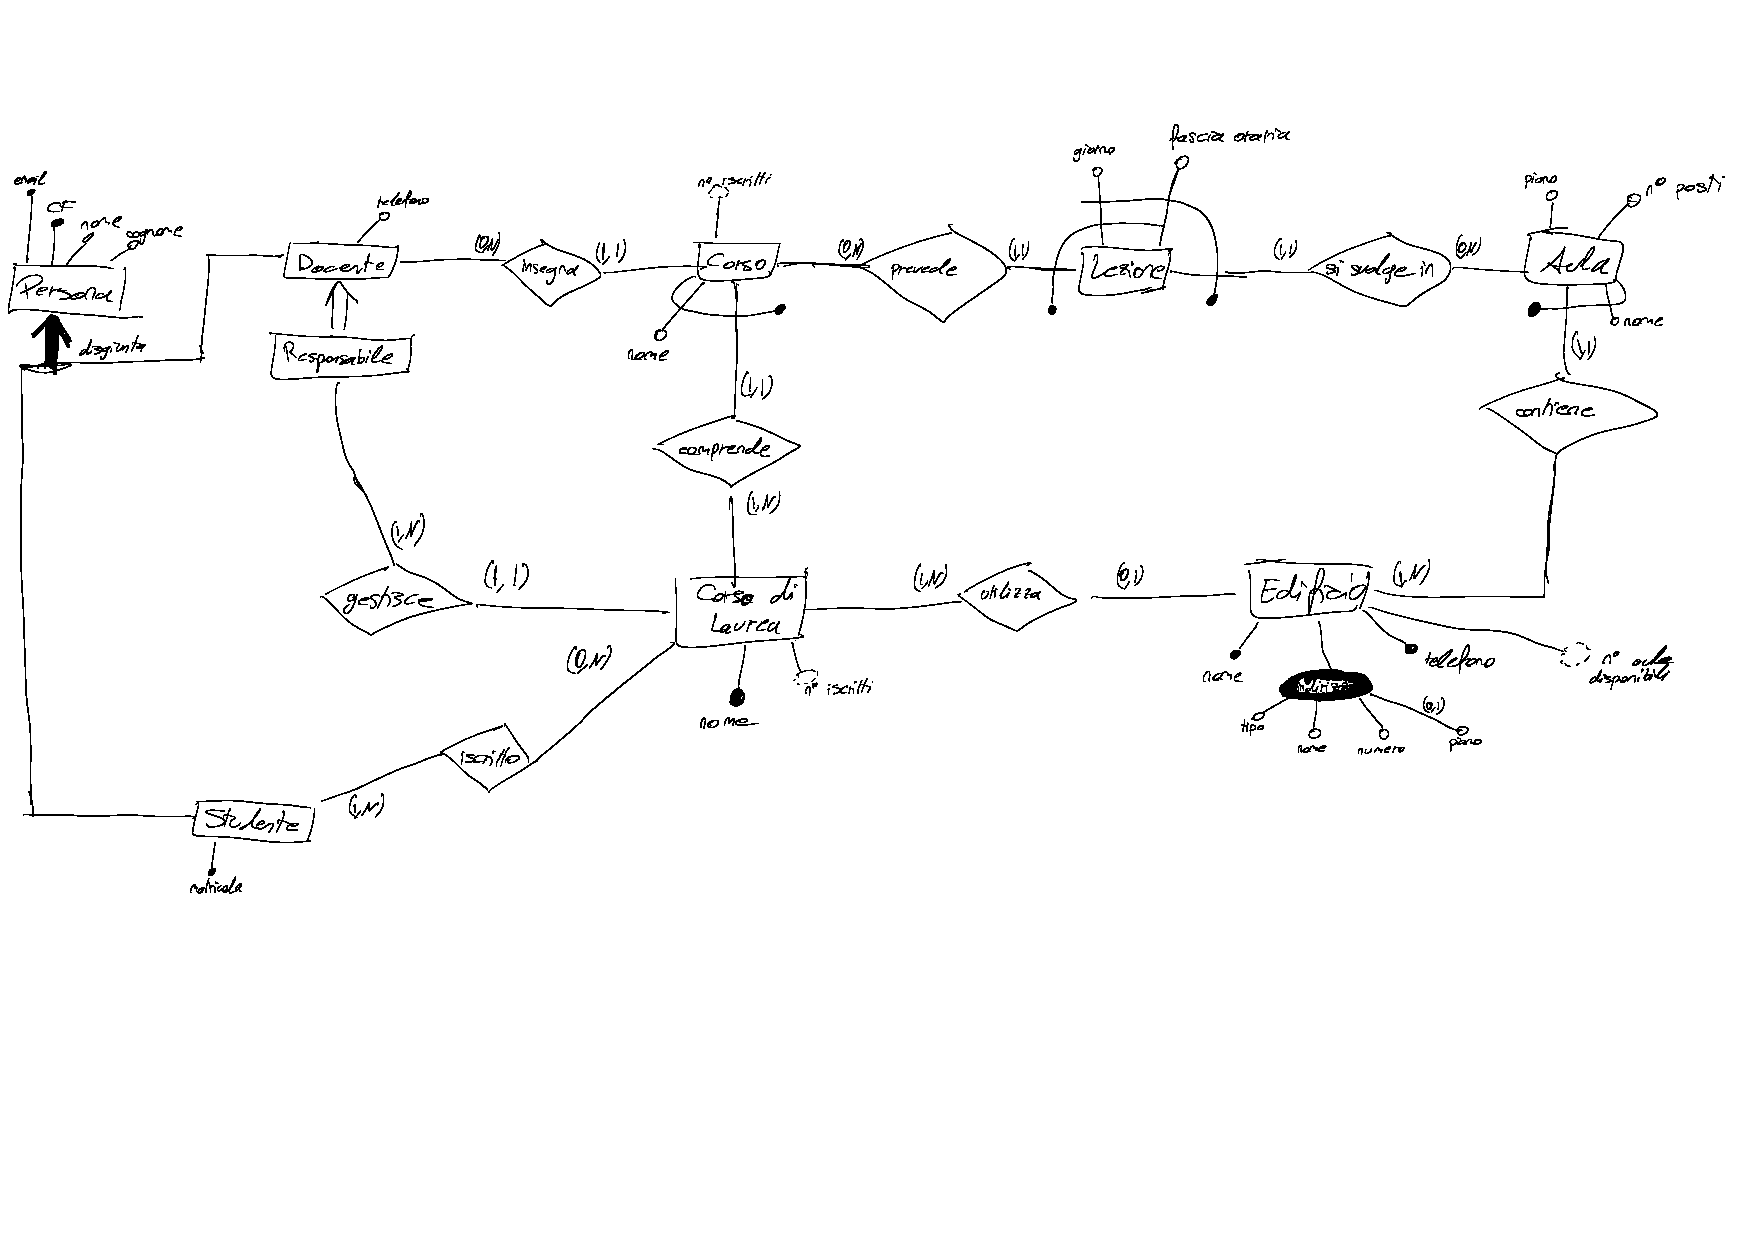
\includegraphics[width=0.95\textwidth]{img/ER Schema.pdf}
    \caption{Schema E-R del sistema per la gestione del calendario delle lezioni}
    \label{fig:er_schema}
\end{figure}


\begin{table}[H]
\centering
\begin{tabularx}{\textwidth}{l l X}
\toprule
\textbf{Entità} & \textbf{Attributo} & \textbf{Tipo} \\
\midrule
Persona & email & tipo stringa con lo stesso formato del email \\
Persona & CF & tipo stringa rappresentante il codice fiscale \\
Persona & nome & tipo stringa alfanumerica \\
Persona & cognome & tipo stringa alfanumerica \\
Docente & telefono & tipo stringa nel formato fisso o mobile italiano, eventualmente comprensivo di prefisso (+39) \\
Studente & matricola & tipo numerico intero maggiore uguale a $0$ \\
Corso & n\textsuperscript{o} iscritti & tipo numerico intero maggiore uguale a $0$ \\
Corso & nome & tipo stringa \\
Corso di Laurea & nome & tipo stringa \\
Corso di Laurea & n\textsuperscript{o} iscritti & tipo numerico intero maggiore uguale a $0$ \\
Lezione & giorno & tipo giorno \\
Lezione & fascia oraria & tipo stringa tale che fascia oraria $\in$ \{prima, seconda, terza, quarta\} \\
Aula & piano & tipo numerico intero maggiore uguale a $-1$ \\
Aula & n\textsuperscript{o} posti & tipo numerico intero maggiore di $0$ \\
Aula & nome & tipo stringa \\
Edificio & nome & tipo stringa \\
Edificio & indirizzo - tipo & tipo stringa tale che tipo $\in \{\text{Via, Piazza, Largo, Viale, Corso, Vicolo}\}$ \\
Edificio & indirizzo - nome & tipo stringa \\
Edificio & indirizzo - numero & tipo numerico intero maggiore uguale a $0$ \\
Edificio & indirizzo - piano & tipo numerico intero maggiore uguale a $-1$ \\
Edificio & recapito telefonico & tipo stringa nel formato fisso o mobile italiano, eventualmente comprensivo di prefisso (+39) \\
Edificio & n\textsuperscript{o} aule disponibili & tipo numerico intero maggiore di $0$ \\

\bottomrule
\end{tabularx}
\caption{Tipi attributi nello schema E-R in Figura~\ref{fig:er_schema}}
\label{tab:attributes_er_schema}
\end{table}



% \subsubsection{Assunzioni sul Contenuto del Database}

% La base di dati è progettata per rappresentare il calendario settimanale delle lezioni relative a uno specifico periodo didattico, però si da la facoltà di memorizzare docenti, edifici, aule e corsi per i quali verranno usati anche in futuro e non necessariamente in tale periodo didattico.

% Per quanto riguarda i corsi di laurea, essi vengono memorizzati esclusivamente se siano attualmente disponibili, per esempio non vengono salvati corsi di laurea per i quali venivano offerti in passato ma che attualmente non vengono più offerti.

% Ogni edificio è associato a un unico corso di laurea. Un edificio può non essere utilizzato per lo svolgimento di lezioni, ma deve comunque essere assegnato a uno specifico corso di laurea.

% % Un corso può non essere associato ad alcun docente nel caso in cui non venga erogato nel periodo didattico considerato; in caso contrario, deve essere associato a un docente.

% Per ogni edificio vengono invece memorizzate tutte le aule (utilizzabili per svolgere lezioni), anche nel caso in cui alcune di esse non siano utilizzate (per rispettare il requisito di memorizzare il numero di aule disponibili).


% \subsubsection{Design Patterns Utilizzati}

% Durante la progettazione dello schema E-R sono stati adottati alcuni design patterns.

% \begin{itemize}
%     \item \textbf{Part-of}: utilizzato per modellare relazioni di composizione, tra Edificio e Aula, Corso e Lezione, Corso di Laurea e Corso.
%     \item \textbf{Reificazione di Relazione}: utilizzato sulla relazione Lezione che l'ha portata a diventare un'entità 

%     \item \textbf{Generalizzazione}:
%     \begin{itemize}
%         \item una generalizzazione totale e disgiunta è utilizzata per specializzare l'entità \emph{Persona} nelle entità \emph{Docente} e
%         \emph{Studente};
%         \item una generalizzazione parziale è utilizzata per rappresentare il ruolo di \emph{Responsabile}, specializzazione dell'entita \emph{Docente}.
%     \end{itemize}
% \end{itemize}


\subsubsection{Strategia di Progettazione}

Lo schema E-R è stato realizzato adottando un approccio \emph{mixed}. In particolare, è stato inizialmente seguito un approccio \emph{top-down} per l'individuazione delle principali entità del dominio; successivamente è stato utilizzato un approccio \emph{inside-out} per integrare le entità e le relazioni necessarie alla realizzazione dello schema finale.


\subsubsection{Vincoli di Integrità}

Lo schema E-R presenta diversi cicli e relazioni che possono essere fonte di probabile inconsistenze; in tale sezione sono stati analizzati per decidere l'eventuale introduzione di vincoli di integrità.


\paragraph{Ciclo \texttt{Corso}-\texttt{Lezione}-\texttt{Aula}-\texttt{Edificio}-\texttt{Corso di Laurea}}
\label{cycle:course_lesson_room_building_degree}

Questo ciclo può generare inconsistenze, poiché lo schema E-R non impedisce strutturalmente di associare a un corso lezioni svolte in aule appartenenti a edifici non associati al relativo corso di laurea oppure a nessun corso di laurea.


\paragraph{Ciclo \texttt{Docente}-\texttt{Corso}-\texttt{Corso di Laurea} - \texttt{Responsabile}}
\label{cycle:teacher_course_degree_resp}

Tale ciclo può essere fonte di inconsistenze, poichè lo schema E-R non impedisce che un responsabile non insegni in alcun corso, oppure che tiene insegnamenti esclusivamente per corsi di laurea differenti da quello che coordina.


\paragraph{Ciclo \texttt{Persona}-\texttt{Docente}-\texttt{Responsabile}-\texttt{Corso di Laurea}-\texttt{Studente}}
\label{cycle:person_teacher_resp_degree_student}

Questo ciclo non è fonte di inconsistenze poiché la generalizzazione tra \texttt{Persona}, \texttt{Docente} e \texttt{Studente} è totale e disgiunta.
Pertanto, non possono esistere istanze che siano contemporaneamente docenti e studenti, e il ciclo non risulta semanticamente rilevante.


\paragraph{Ciclo \texttt{Docente}-\texttt{Corso}-\texttt{Lezione}-\texttt{Aula}-\texttt{Edificio}-\texttt{Corso di Laurea}-\texttt{Responabile}}
\label{cycle:teacher_course_lesson_room_building_degree_resp}

Oltre alle considerazioni svolte nel \nameref{cycle:course_lesson_room_building_degree}, in questo ciclo non è necessario aggiungere ulteriori vincoli di integrità.


\paragraph{Ciclo \texttt{Persona}-\texttt{Docente}-\texttt{Corso}-\texttt{Corso di Laurea}-\texttt{Studente}}

Per le stesse considerazioni svolte nel \nameref{cycle:person_teacher_resp_degree_student} tale ciclo non è fonte di probabili inconsistenze considerando il fatto che la generalizzazione è disgiunta.


\paragraph{Ciclo \texttt{Persona}-\texttt{Docente}-\texttt{Corso}-\texttt{Lezione}-\texttt{Aula}-\texttt{Edificio}-\texttt{Corso di Laurea}-\texttt{Studente}}

Oltre alle considerazioni svolte sul ciclo \nameref{cycle:teacher_course_lesson_room_building_degree_resp}, questo ciclo non introduce ulteriori vincoli di integrità e può essere considerato non rilevante dal punto di vista semantico, in quanto la generalizzazione totale e disgiunta elimina la possibilità di sovrapposizione tra i ruoli coinvolti tra le entità studente e docente.


\paragraph{Vincoli di Integrità Aggiuntivi}
\label{sec:integrity_constraints}

L'analisi dei cicli presenti nello schema E-R ha evidenziato alcuni vincoli semantici che non possono essere rappresentati direttamente tramite costrutti dello schema E-R relativamente al \nameref{cycle:course_lesson_room_building_degree} e \nameref{cycle:teacher_course_degree_resp}.
Tali vincoli vengono esplicitati come vincoli di integrità aggiuntivi.


\begin{enumerate}[label=\textbf{Vincolo Integrità \arabic*:}, ref=\textbf{Vincolo Integrità \arabic*}, series=integrity-constraints, leftmargin=*]
    \item Le lezioni di un corso devono svolgersi esclusivamente in aule appartenenti a edifici associati al corso di laurea a cui il corso appartiene;
    \label{ic:building_course}
    
    \item Il docente responsabile di un corso di laurea deve insegnare almeno un corso appartenente a tale corso di laurea.
    \label{ic:responsable_course}
\end{enumerate}


\subsubsection{Ridondanze}
\label{sec:all_redundancy}

Dallo schema E-R si possono notare le seguenti ridondanze:

\begin{itemize}
    \item l'attributo \texttt{n\textsuperscript{o} iscritti} nelle entità \texttt{Corso di Laurea} e \texttt{Corso} che identificano rispettivamente il numero totale di studenti iscritti al corso di laurea e al corso di laurea del associato corso;
    \item l'attributo \texttt{n\textsuperscript{o} aule disponibili} nel entità \texttt{Edificio} che identifica il numero totale di aule utilizzabili per fare lezione nel edificio.
\end{itemize}


\subsubsection{Politiche di Cancellazione sulle Entità}
\label{sec:entity_deletion_policies}

Al fine di dettagliare i vincoli di partecipazione e di ciclo di vita non esprimibili graficamente nel diagramma E-R, viene di seguito definito il comportamento del sistema in caso di eliminazione di un'istanza per ciascuna entità.

\begin{description}[leftmargin=*]

    \item[Eliminazione di un docente:] \hfill \\
    La rimozione di un docente è vincolata ai suoi corsi: può essere eseguita esclusivamente se il docente non risulta titolare di alcun corso attivo. In caso contrario, l'operazione è bloccata; per procedere alla cancellazione, è necessario assegnare preventivamente un nuovo docente ai corsi interessati.

    \item[Eliminazione di un responsabile:] \hfill \\
    Un responsabile di un corso di laurea non può essere rimosso direttamente dal sistema. La cancellazione è subordinata alla revoca dal insegnamento di tutti i suoi corsi e all'assegnazione di un altro responsabile al corso di laurea per il quale risulta responsabile.

    \item[Eliminazione di uno studente:] \hfill \\
    L'istanza relativa a uno studente può essere rimossa dal sistema senza alcun vincolo restrittivo o effetto collaterale sulle altre entità.

    \item[Eliminazione di un corso:] \hfill \\
    La rimozione di un corso comporta la cancellazione automatica e in cascata di tutte le singole lezioni ad esso associate e pianificate nel calendario.

    \item[Eliminazione di un corso di laurea:] \hfill \\
    La rimozione di un corso di laurea comporta la cancellazione automatica di tutti i corsi ad esso afferenti e la contestuale rimozione di tutte le relative iscrizioni. Inoltre, per preservare il vincolo di partecipazione totale degli studenti, l'operazione estende la cancellazione in cascata a tutti quei studenti la cui unica iscrizione attiva era associata al corso di laurea eliminato. Al contrario, la sua rimozione non ha alcun effetto sui edifici: gli edifici utilizzati per lo svolgimento delle lezioni non devono essere rimossi.

    \item[Eliminazione di una lezione:] \hfill \\
    La rimozione di una singola lezione dal calendario può essere effettuata liberamente, senza alcuna limitazione o conseguenza sistemica sul resto della base di dati.

    \item[Eliminazione di un'aula:] \hfill \\
    La rimozione di un'aula è consentita solo se non vi sono lezioni programmate al suo interno. Qualora siano presenti delle lezioni, l'operazione viene bloccata finché queste non vengono preventivamente ricollocate in altre aule.

    \item[Eliminazione di un edificio:] \hfill \\
    La rimozione di un edificio comporta necessariamente la cancellazione automatica e in cascata di tutte le aule in esso strutturalmente contenute.

\end{description}


\subsection{Risultati Progettazione Concettuale}

Al termine di tale fase gli artefatti principali sono lo schema ER in Figura~\ref{fig:er_schema} con le informazioni sui tipi dei attributi presenti nella Tabella~\ref{tab:attributes_er_schema}, le operazioni nella sezione \nameref{sec:operations}, tutti i vincoli di integrità nella sezione~\nameref{sec:integrity_constraints} e infine le politiche di rimozione delle entità nella sezione~\nameref{sec:entity_deletion_policies}.



\section{Progettazione Logica}

\subsection{Ristrutturazione dello Schema E-R}

\subsubsection{Rimozione degli Attributi Composti}

Dallo schema E-R in Figura~\ref{fig:er_schema} risulta la presenza di un unico attributo composto (\texttt{indirizzo} nell'entità \texttt{Edificio}). Per la gestione di tale attributo si è deciso di rappresentarlo come attributo atomico di tipo stringa, che rispetti il formato di un indirizzo italiano.

Tale scelta è motivata dal fatto che l'indirizzo deve essere memorizzato al solo fine di identificare la posizione, e non sono previste operazioni o requisiti che richiedano la manipolazione separata delle singole componenti dell'attributo.


\subsubsection{Rimozione delle Generalizzazioni}

Dallo schema E-R in Figura~\ref{fig:er_schema} risultano presenti due generalizzazioni, che sono state rimosse come mostrato in Figura~\ref{fig:generalization_removed}.

\begin{figure}[H]
    \centering
    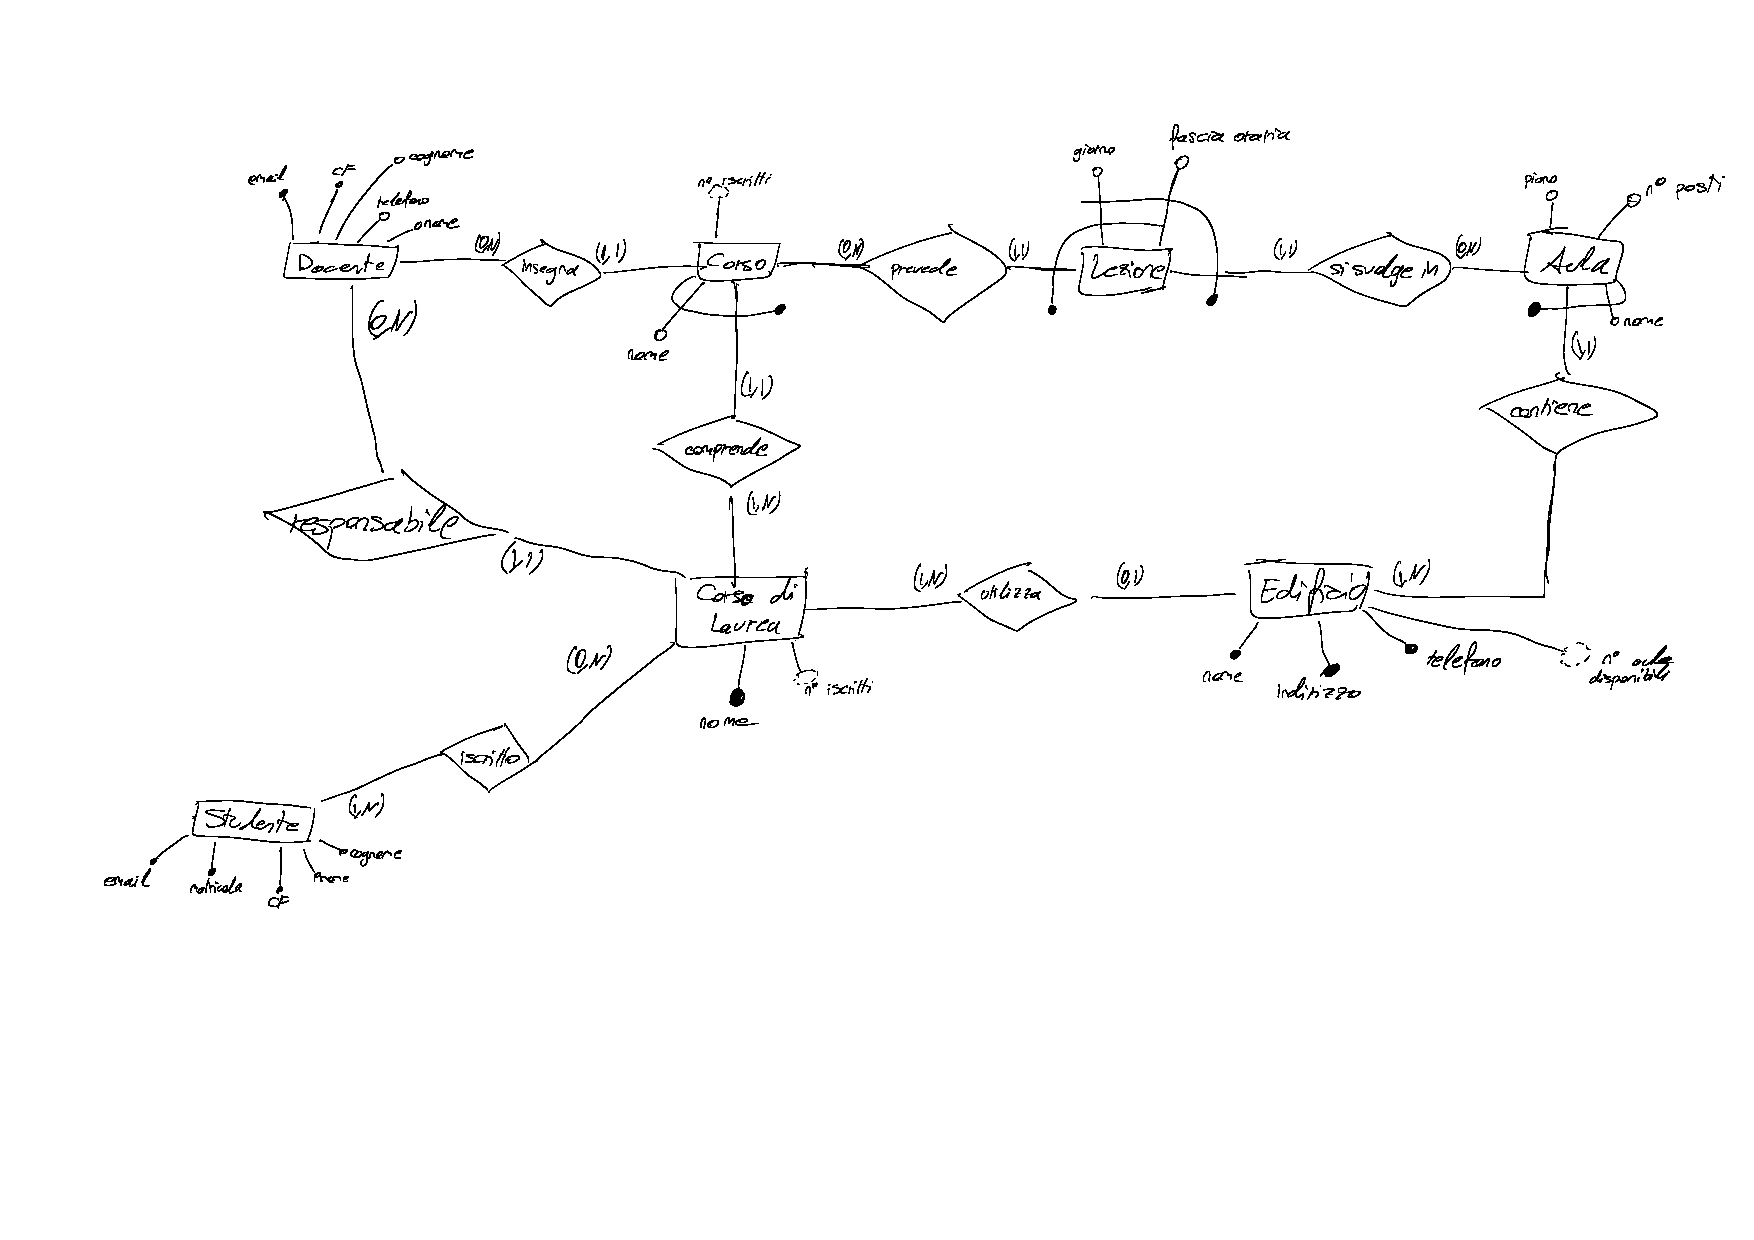
\includegraphics[width=1\linewidth]{img/Removed Generalizations ER Schema.pdf}
    \caption{Schema ER privo di generalizzazioni}
    \label{fig:generalization_removed}
\end{figure}

Nella generalizzazione tra \texttt{Persona}, \texttt{Docente} e \texttt{Studente}, si è deciso di rimuovere l'entità padre \texttt{Persona}, mantenendo le entità figlie. Tale scelta è giustificata dal fatto che la generalizzazione è totale e disgiunta e non esistono operazioni che coinvolgano direttamente l'entità padre ma solo operazioni che coinvolgono separatamente l'entità \texttt{Docente} e l'entità \texttt{Studente}. Tale scelta comporta l'introduzione del vincolo di integrità

\begin{enumerate}[label=\textbf{Vincolo Integrità \arabic*}:, ref=\textbf{Vincolo Integrità \arabic*}, resume=integrity-constraints, leftmargin=*]
    \item Le entità \texttt{Docente} e \texttt{Studente} sono disgiunte: un individuo può appartenere a una sola delle due entità.
    \label{ic:student_teacher}
\end{enumerate}

Nella generalizzazione tra \texttt{Docente} e \texttt{Responsabile}, essendo la generalizzazione parziale e non essendoci attributi aggiuntivi nell'entità \texttt{Responsabile} (in quanto rappresenta un ruolo del docente), si è deciso di accorpare l'entità \texttt{Responsabile} con l'entità \texttt{Docente} e modellare il ruolo tramite la relazione \texttt{responsabile}.

Questa scelta consente di semplificare lo schema E-R, senza introdurre valori \texttt{NULL} e senza la necessità di introdurre ulteriori vincoli di integrità.


\subsubsection{Disaccoppiamento/Aggregazione di Entità e Relazioni}

Dall'analisi dello schema E-R e delle operazioni non emergono esigenze di disaccoppiamento o aggregazione di entità o relazioni.


\subsubsection{Analisi delle Ridondanze}

Tra le ridondanze individuate (Sezione~\nameref{sec:all_redundancy}), si è scelto di analizzare in dettaglio quella relativa all'attributo \texttt{n\textsuperscript{o} iscritti} nell'entità \texttt{Corso di Laurea}.

Per quanto riguarda l'attributo \texttt{n\textsuperscript{o} aule disponibili} e l'attributo \texttt{n\textsuperscript{o} iscritti} nell'entità \texttt{Corso}, si è deciso di non mantenerli nello schema E-R, in quanto non risultano rilevanti rispetto alle operazioni considerate e non giustificano l'introduzione di ridondanze.


\paragraph{Analisi delle Performance}

Vengono riportate le informazioni relative ai volumi dei dati e alle frequenze delle operazioni.

\begin{table}[H]
    \centering
    
    \begin{subtable}{0.48\textwidth}
        \centering
    
        \begin{tabular}{ l l l }
            \toprule
            \textbf{Concetto} & \textbf{Tipo} & \textbf{Volume} \\
            \midrule
            Persona & E & 1.600 \\
            Studente & E & 1.500 \\
            Docente & E & 100 \\
            Corso di Laurea & E & 10 \\
            Corso & E & 200 \\
            Lezione & E & 7.200 \\
            Aula & E & 240 \\
            Edificio & E & 12 \\
            Iscritto & R & 2.000 \\
            Responsabile & R & 10 \\
            Insegna & R & 200 \\
            Utilizza & R & 12 \\
            Comprende & R & 200 \\
            Contiene & R & 240 \\
            Prevede & R & 7.200 \\
            Si svolte in & R & 7.200 \\
            \bottomrule
        \end{tabular}
    
        \caption{Tabella dei volumi}
        \label{tab:volumes}
    
    \end{subtable}
    \hfill
    \begin{subtable}{0.48\textwidth}
        \centering
        \begin{tabular}{l l l }
            \toprule
            \textbf{Operazione} & \textbf{Tipo} & \textbf{Frequenza} \\
            \midrule
            \ref{op:insert_student} & I & 500 / anno \\
            \ref{op:get_info_degree} & I & 10 / giorno \\
            \ref{op:transfer_student} & I & 30 / anno \\
            \ref{op:find_teachers_by_responsible} & I & \\
            \ref{op:find_course_max_rooms} & I & \\
            \ref{op:find_courses_covering_rooms} & I & \\
            \ref{op:find_students_by_teacher} & I \\
            \ref{op:find_course_in_same_rooms} & I & \\
            \ref{op:create_building} & I & \\
            \ref{op:create_degree} & I & \\
            \ref{op:remove_room} & I & \\
            \ref{op:change_room_lesson} & I & \\
            \bottomrule
        \end{tabular}
        \caption{Tabella delle operazioni}
        \label{tab:operations}
    \end{subtable}
\end{table}


\paragraph{Sottoschema di riferimento}\mbox{}\\

\begin{figure}[H]
    \centering
    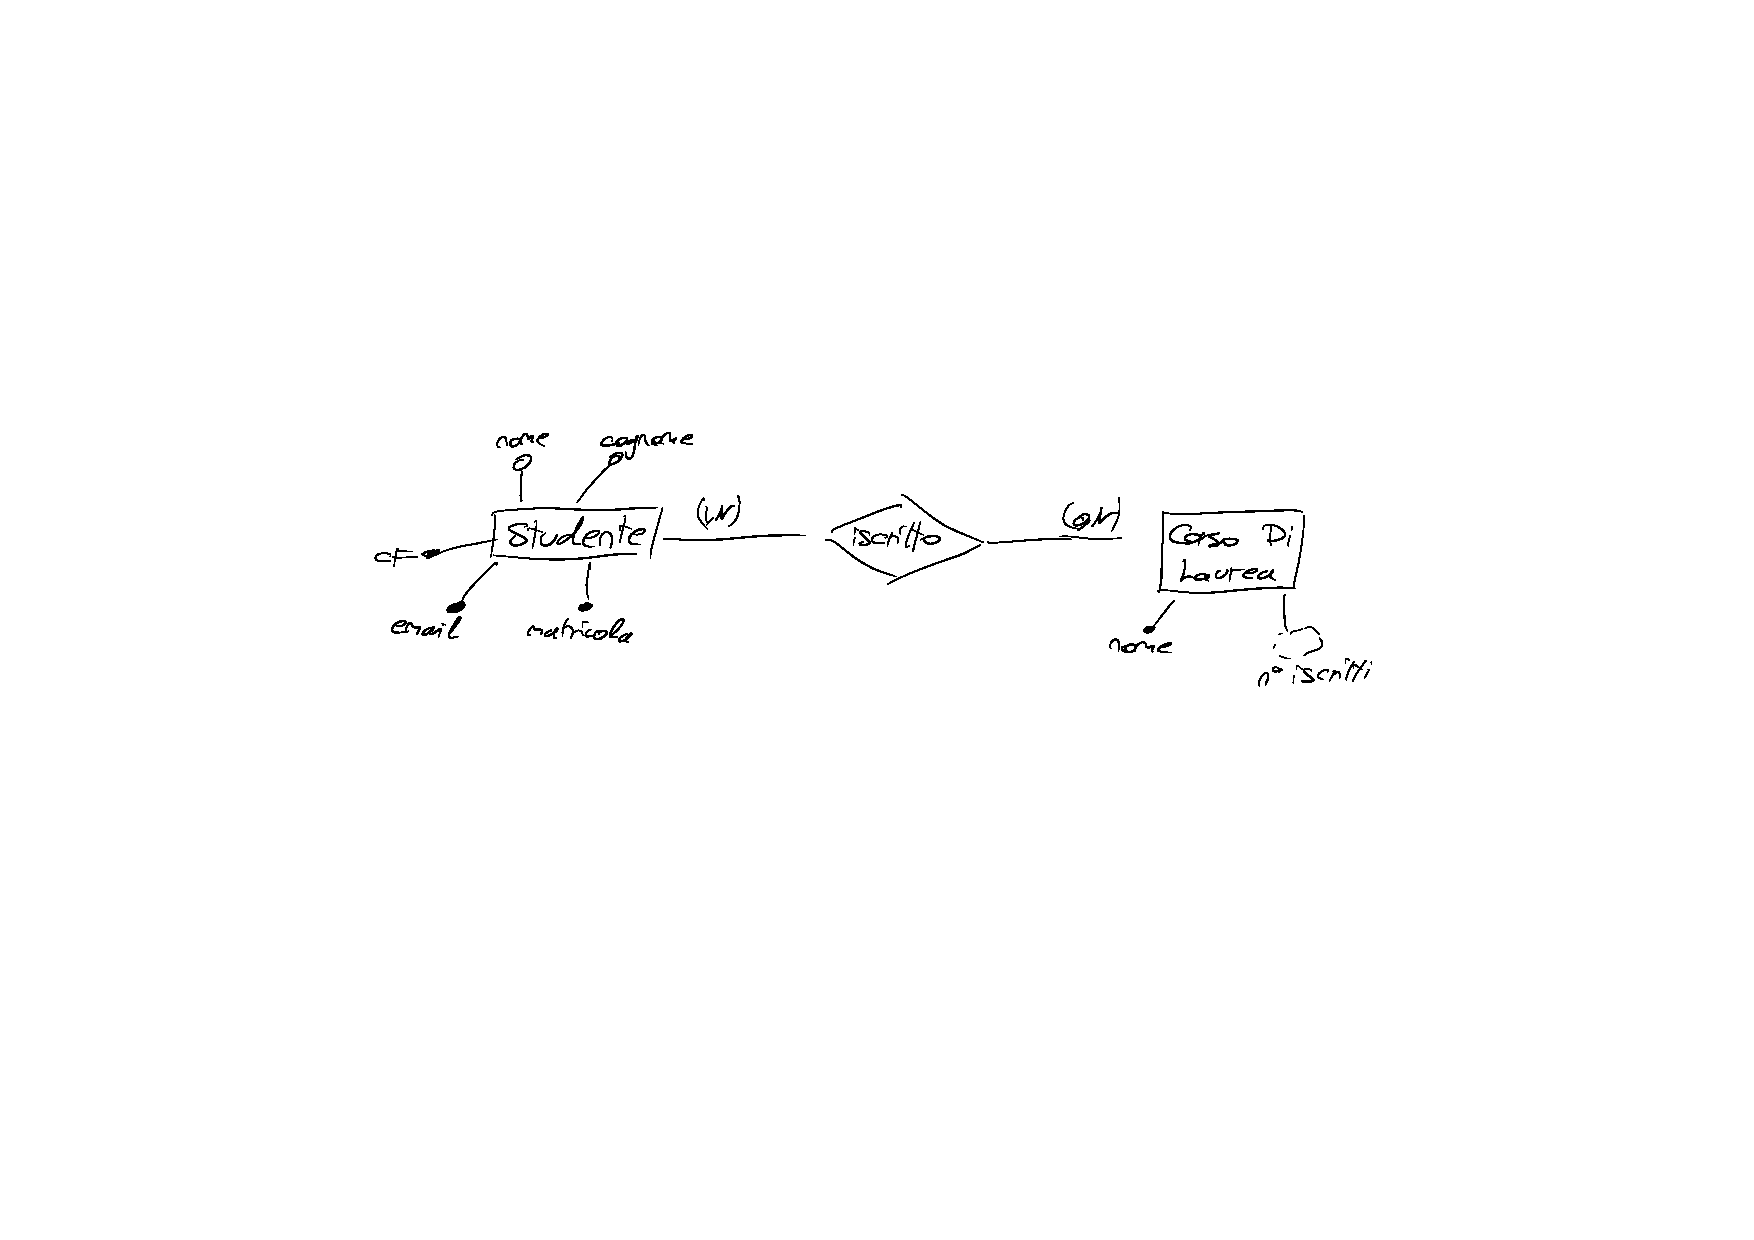
\includegraphics[width=0.7\textwidth, trim={200pt, 200pt, 200pt, 200pt}]{img/Redundancy ER Schema.pdf}
    \caption{Sotto-schema E-R per l'analisi delle ridondanze sul attributo \texttt{n\textsuperscript{o} iscritti}}
    \label{fig:er_redundancy_subschema}
\end{figure}


\paragraph{Volumi e operazioni}\mbox{}\\

\begin{table}[H]
    \centering
    
    \begin{subtable}{0.48\textwidth}
        \centering
        \begin{tabular}{l l l }
            \toprule
            \textbf{Concetto} & \textbf{Tipo} & \textbf{Volume} \\
            \midrule
            Corso di Laurea & E & 10 \\
            Studente & E & 1.500 \\
            Iscritto & R & 2.000 \\
            \bottomrule
        \end{tabular}
        \caption{Tabella dei volumi}
        \label{tab:redundancy_volumes}
    \end{subtable}
    \hfill
    \begin{subtable}{0.48\textwidth}
        \centering
        \begin{tabular}{l l l }
            \toprule
            \textbf{Operazione} & \textbf{Tipo} & \textbf{Frequenza} \\
            \midrule
            \ref{op:insert_student} & I & 500 / anno \\
            \ref{op:get_info_degree} & I & 10 / giorno \\
            \ref{op:transfer_student} & I & 30 / anno \\
            \bottomrule
        \end{tabular}
        \caption{Tavola delle operazioni}
        \label{tab:redundancy_operations}
    \end{subtable}
\end{table}


\paragraph{Presenza delle Ridondanze}

In questa sezione viene analizzato il costo delle operazioni nel caso in cui l'attributo derivato \texttt{n\textsuperscript{o} iscritti} sia mantenuto nell'entità \texttt{Corso di Laurea}. Le tabelle seguenti riportano gli accessi alle entità e alle relazioni coinvolte in ciascuna operazione.

\begin{table}[H]
    \centering
    \begin{subtable}{0.48\textwidth}
        \centering
        \begin{tabular}{l l l l}
            \toprule
            \textbf{Concetto} & \textbf{Tipo} & & \textbf{Accessi} \textbf{Tipo} \\
            \midrule
            Studente & E & 1 & W \\
            Iscritto & R & 1 & W \\
            Corso di Laurea & E & 1 & R \\
            Corso di Laurea & E & 1 & W \\
            \bottomrule
        \end{tabular}
        \caption{Tabella accessi \ref{op:insert_student}}
        \vspace{1cm}
        \begin{tabular}{l l l l }
            \toprule
            \textbf{Concetto} & \textbf{Tipo} & & \textbf{Accessi} \textbf{Tipo} \\
            \midrule
            Corso di Laurea & E & 1 & R \\
            \bottomrule
        \end{tabular}
        \caption{Tabella accessi \ref{op:get_info_degree}}
    \end{subtable}
    \hfill
    \begin{subtable}{0.48\textwidth}
        \centering
        \begin{tabular}{l l l l}
            \toprule
            \textbf{Concetto} & \textbf{Tipo} & & \textbf{Accessi} \textbf{Tipo} \\
            \midrule
            Iscritto & R & 1 & R \\
            Iscritto & R & 1 & W \\
            Corso di Laurea & E & 1 & R \\
            Corso di Laurea & E & 1 & W \\
            Corso di Laurea & E & 1 & R \\
            Corso di Laurea & R & 1 & W \\
            \bottomrule
        \end{tabular}
        \caption{Tabella accessi \ref{op:transfer_student}}
    \end{subtable}
\end{table}


\paragraph{Assenza delle Ridondanze}

In questa sezione viene analizzato il costo delle stesse operazioni nel caso in cui l'attributo derivato \texttt{n\textsuperscript{o} iscritti} non venga introdotto, rendendo necessario il calcolo del numero di studenti iscritti tramite l'accesso alla relazione \texttt{Iscritto}.

\begin{table}[H]
    \centering
    \begin{subtable}{0.48\textwidth}
        \centering
        \begin{tabular}{l l l l}
            \toprule
            \textbf{Concetto} & \textbf{Tipo} & & \textbf{Accessi} \textbf{Tipo} \\
            \midrule
            Studente & E & 1 & W \\
            Iscritto & R & 1 & W \\
            \bottomrule
        \end{tabular}
        \caption{Tabella accessi \ref{op:insert_student}}
        \vspace{1cm}
        \begin{tabular}{l l l l}
            \toprule
            \textbf{Concetto} & \textbf{Tipo} & & \textbf{Accessi} \textbf{Tipo} \\
            \midrule
            Corso di Laurea & E & 1 & R \\
            Iscritti & R & 200 & R \\
            \bottomrule
        \end{tabular}
        \caption{Tabella accessi \ref{op:get_info_degree}}
    \end{subtable}
    \hfill
    \begin{subtable}{0.48\textwidth}
        \centering
        \begin{tabular}{l l l l}
            \toprule
            \textbf{Concetto} & \textbf{Tipo} & & \textbf{Accessi} \textbf{Tipo} \\
            \midrule
            Iscritto & R & 1 & R \\
            Iscritto & R & 1 & W \\
            \bottomrule
        \end{tabular}
        \caption{Tabella accessi \ref{op:transfer_student}}
    \end{subtable}
\end{table}


\paragraph{Analisi dei Costi}

In questa sezione viene confrontato il costo complessivo delle operazioni considerate nei due casi: presenza e assenza della ridondanza relativa al numero di studenti iscritti a un corso di laurea.
Il costo è espresso in termini di numero di letture (costo = 1) e scritture (costo = 2) sulle entità e relazioni coinvolte, pesate in base alla frequenza delle operazioni.


\subparagraph{Presenza di Ridondanza}

\begin{itemize}
    \item l'operazione \ref{op:insert_student} richiede 1 lettura e 3 scritture;
    \item l'operazione \ref{op:get_info_degree} richiede 1 lettura;
    \item l'operazione \ref{op:transfer_student} richiede 3 letture e 3 scritture.
\end{itemize}


\subparagraph{Assenza di Ridondanza}

\begin{itemize}
    \item l'operazione \ref{op:insert_student} richiede 2 scritture;
    \item l'operazione \ref{op:get_info_degree} richiede 201 letture;
    \item l'operazione \ref{op:transfer_student} richiede 1 lettura e 1 scrittura.
\end{itemize}


\subparagraph{Costo Totale}

Tenendo conto delle frequenze delle operazioni, il costo complessivo risulta pari a:
$$ \text{Costo con ridondanza} = 500*7+3650+30*9 = 7.420$$
$$ \text{Costo senza ridondanza} = 500*4+3650*201+30*3 = 735.740 $$


\paragraph{Conclusioni}
Si conclude che il mantenimento della ridondanza risulta conveniente, in quanto riduce in modo significativo il costo complessivo delle operazioni.


\subsubsection{Scelta degli Identificatori Principali}

\begin{table}[H]
    \centering
    \begin{tabular}{l l}
    \toprule
    \textbf{Entità} & \textbf{Identificatore scelto} \\
    \midrule
    Studente & CF \\
    Docente & CF \\
    Corso di Laurea & nome \\
    Corso & (nome, corso di laurea) \\
    Aula & (nome, edificio) \\
    Edificio & nome \\
    Lezione & (giorno, fascia oraria, corso) \\
    \bottomrule
    \end{tabular}
\end{table}


\subsection{Schema Relazionale}
\label{sec:logical_schema}

Di seguito si riporta lo schema logico relazionale derivato dallo schema E-R ristrutturato, integrato con le politiche di gestione delle cancellazioni sulle chiavi esterne.

\begin{description}[leftmargin=*]

\item[\texttt{Docente(CF, nome, cognome, email, telefono)}] \hfill \\
\textbf{PK:} CF \\
\textbf{VNN:} \{email, nome, cognome, telefono\} \\
\textbf{UNIQUE:} \{email\}


\item[\texttt{Studente(CF, matricola, nome, cognome, email)}] \hfill \\
\textbf{PK:} CF \\
\textbf{VNN:} \{matricola, nome, cognome, email\} \\
\textbf{UNIQUE:} \{matricola, email\}

\begin{enumerate}[label=\textbf{Vincolo Integrità \arabic*}:, ref=\textbf{Vincolo Integrità \arabic*}, resume=integrity-constraints, leftmargin=*]
    \item Ogni studente deve essere iscritto ad almeno un corso di laurea. Per preservare tale vincolo, la cancellazione di tutte le iscrizioni di uno studente deve comportarne la sua rimozione.
    \label{ic:student_degree_participation}
\end{enumerate}


\item[\texttt{Corso di Laurea(nome, n\textsuperscript{o} iscritti, responsabile)}] \hfill \\
\textbf{PK:} nome \\
\textbf{VNN:} \{n\textsuperscript{o} iscritti, responsabile\} \\
\textbf{FK}: \{(responsabile $\rightarrow$ Docente(CF))\} \\
\textbf{Politiche di Integrità Referenziale:}
\begin{description}[leftmargin=*]
    \item Non è possibile eliminare un docente se ricopre la carica di responsabile del corso di laurea. La rimozione è bloccata finché non viene nominato un sostituto.
\end{description}

\begin{enumerate}[label=\textbf{Vincolo Integrità \arabic*}:, ref=\textbf{Vincolo Integrità \arabic*}, resume=integrity-constraints, leftmargin=*]
    \item Ogni corso di laurea deve presentare almeno un corso
    \label{ic:degree_course_participation}    
\end{enumerate}


\item[\texttt{Corso(nome, corso di laurea, docente)}] \hfill \\
\textbf{PK:} (nome, corso di laurea) \\
\textbf{VNN:} \{docente\} \\
\textbf{FK:} \{(corso di laurea $\rightarrow$ Corso di Laurea(nome)), (docente $\rightarrow$ Docente(CF))\} \\
\textbf{Politiche di Integrità Referenziale:}
\begin{description}[leftmargin=*]
    \item La cancellazione di un corso di laurea comporta la rimozione automatica di tutti i relativi corsi afferenti.
    \item La rimozione di un docente è bloccata. Il corso deve essere riassegnato prima di poter cancellare il docente.
\end{description}


\item[\texttt{Iscritto(studente, corso di laurea)}] \hfill \\
\textbf{PK:} (studente, corso di laurea) \\
\textbf{FK:} \{(studente $\rightarrow$ Studente(CF)), (corso di laurea $\rightarrow$ Corso di Laurea(nome))\} \\
\textbf{Politiche di Integrità Referenziale:}
\begin{description}[leftmargin=*]
    \item La cancellazione di uno studente comporta la rimozione di tutte le sue iscrizioni.
    \item La rimozione di un corso di laurea comporta la cancellazione di tutte le iscrizioni relative a tale corso di laurea.
\end{description}


\item[\texttt{Edificio(nome, indirizzo, telefono, corso di laurea)}] \hfill \\
\textbf{PK:} nome \\
\textbf{VNN:} \{indirizzo, telefono\} \\
\textbf{UNIQUE:} \{indirizzo, telefono\} \\
\textbf{FK:} (corso di laurea $\rightarrow$ Corso di Laurea(nome)) \\
\textbf{Politiche di Integrità Referenziale:}
\begin{description}[leftmargin=*]
    \item In caso di rimozione di un corso di laurea, l'assegnazione dei relativi edifici deve essere annullata, in modo da renderli nuovamente disponibili per altri corsi di laurea.
\end{description}

\begin{enumerate}[label=\textbf{Vincolo Integrità \arabic*}:, ref=\textbf{Vincolo Integrità \arabic*}, resume=integrity-constraints, leftmargin=*]
    \item Ogni edificio deve contenere almeno un'aula
    \label{ic:building_room_participation}
\end{enumerate}


\item[\texttt{Aula(nome, edificio, piano, n\textsuperscript{o} posti)}] \hfill \\
\textbf{PK:} (nome, edificio) \\
\textbf{VNN:} \{piano, n\textsuperscript{o} posti\} \\
\textbf{FK:} \{(edificio $\rightarrow$ Edificio(nome))\} \\
\textbf{Politiche di Integrità Referenziale:}
\begin{description}[leftmargin=*]
    \item L'eliminazione di un edificio comporta la cancellazione automatica di tutte le sue aule.
\end{description}


\item[\texttt{Lezione(corso, corso di laurea, giorno, fascia oraria, aula, edificio)}] \hfill \\
\textbf{PK:} (corso, corso di laurea, giorno, fascia oraria)\\
\textbf{UNIQUE:} \{(giorno, fascia oraria, aula, edificio)\} \\
\textbf{VNN:} \{aula, edificio\} \\
\textbf{FK:} \{(corso, corso di laurea $\rightarrow$ Corso(nome, corso di laurea)), (aula, edificio $\rightarrow$ Aula(nome, edificio))\} \\
\textbf{Politiche di Integrità Referenziale:}
\begin{description}[leftmargin=*]
    \item La cancellazione di un singolo corso rimuove automaticamente tutte le sue lezioni programmate nel calendario.
    \item La rimozione di un'aula è bloccata qualora vi siano lezioni pianificate al suo interno, forzando lo spostamento delle lezioni in altre aule.
\end{description}

\end{description}


\subsection{Risultati Progettazione Logica}

Oltre allo schema relazionale implementato nella sezione~\nameref{sec:logical_schema} la progettazione logica definisce i seguenti componenti necessari a garantire l'integrità e la corretta gestione dei dati.


\subsubsection{Vincoli di Integrità}

Al fine di mantenere la consistenza della base di dati, sono stati definiti i seguenti vincoli:

\begin{itemize}
    \item \ref{ic:building_course}: le lezioni di un corso devono svolgersi esclusivamente in aule appartenenti a edifici associati al corso di laurea a cui il corso appartiene.
    \item \ref{ic:responsable_course}: il docente responsabile di un corso di laurea deve insegnare almeno un corso appartenente a tale corso di laurea.
    \item \ref{ic:student_teacher}: un docente non può essere anche uno studente e, viceversa, uno studente non può essere anche un docente.
    \item \ref{ic:student_degree_participation}: ogni studente deve essere iscritto ad almeno un corso di laurea. La rimozione di tutte le iscrizioni di uno studente deve comportarne la sua rimozione.
    \item \ref{ic:degree_course_participation}: ogni corso di laurea deve comprendere almeno un corso.
    \item \ref{ic:building_room_participation}: per ogni edificio deve esistere almeno un'aula ad esso associata.
\end{itemize}


\subsubsection{Regole di Derivazione}

Al fine di ottimizzare le prestazioni delle query, è stato introdotto nell'entità \texttt{Corso di Laurea} l'attributo derivato \texttt{n\textsuperscript{o} iscritti}. La relativa regola di derivazione prevede che il valore sia calcolato come conteggio di tutti gli studenti iscritti al medesimo corso di laurea.


\subsubsection{Domini degli Attributi}

Nella Tabella~\ref{tab:attributes_rel_schema} sono riportati i domini associati agli attributi delle relazioni dello schema logico relazionale.

\begin{table}[H]
\centering
\begin{tabularx}{\textwidth}{l l X}
    \toprule
    \textbf{Entità} & \textbf{Attributo} & \textbf{Tipo} \\
    \midrule
    Persona & email & tipo stringa, con lo stesso formato del email, con lunghezza massima pari a 100 \\
    Persona & CF & tipo stringa rappresentante il codice fiscale \\
    Persona & nome & tipo stringa alfanumerica, con lunghezza massima pari a 50 \\
    Persona & cognome & tipo stringa alfanumerica, con lunghezza massima pari a 50 \\
    Docente & telefono & tipo stringa nel formato fisso o mobile italiano, eventualmente comprensivo di prefisso (+39) \\
    Studente & matricola & tipo numerico intero maggiore uguale a $0$ \\
    Corso & n\textsuperscript{o} iscritti & tipo numerico intero maggiore uguale a $0$ \\
    Corso & nome & tipo stringa, con lunghezza massima pari a 100 \\
    Corso di Laurea & nome & tipo stringa, con lunghezza massima pari a 100 \\
    Corso di Laurea & n\textsuperscript{o} iscritti & tipo numerico intero maggiore uguale a $0$ \\
    Lezione & giorno & tipo giorno \\
    Lezione & fascia oraria & tipo stringa tale che fascia oraria $\in$ \{prima, seconda, terza, quarta\} \\
    Aula & piano & tipo numerico intero maggiore uguale a $-1$ \\
    Aula & n\textsuperscript{o} posti & tipo numerico intero intero maggiore di $0$ \\
    Aula & nome & tipo stringa, con lunghezza massima pari a 100 \\
    Edificio & nome & tipo stringa, con lunghezza massima pari a 100 \\
    Edificio & indirizzo & stringa conforme al formato di un indirizzo italiano, con lunghezza massima pari a 100 \\
    Edificio & recapito telefonico & tipo stringa nel formato fisso o mobile italiano, eventualmente comprensivo di prefisso (+39) \\
    Edificio & n\textsuperscript{o} aule disponibili & tipo numerico intero maggiore di $0$ \\
    
    \bottomrule
\end{tabularx}
\caption{Domini attributi dello schema logico relazionale}
\label{tab:attributes_rel_schema}
\end{table}


\section{Implementazione dei vincoli di integrità}

Durante l'implementazione della base di dati è stata realizzata soltanto una parte dei vincoli di integrità individuati durante le fasi di progettazione concettuale e logica.

In particolare, sono stati implementati i seguenti vincoli di integrità:

\begin{itemize}
    \item \ref{ic:student_teacher}: un docente non può essere contemporaneamente anche uno studente e viceversa;
    \item \ref{ic:student_degree_participation}: ogni studente deve essere iscritto ad almeno un corso di laurea. La rimozione di tutte le iscrizioni di uno studente deve comportarne la sua rimozione.
\end{itemize}

Inoltre, è stato implementato un trigger per la gestione automatica dell'attributo \texttt{n\textsuperscript{o} iscritti} dell'entità \texttt{Corso di Laurea}.

I restanti vincoli di integrità non sono stati implementati direttamente all'interno della base di dati.


\subsection{\ref{ic:building_course}}

Tale vincolo richiede che le lezioni di un corso si svolgano esclusivamente in aule appartenenti a edifici associati al corso di laurea a cui il corso appartiene.

L'implementazione del vincolo sarebbe stata realizzata mediante diversi trigger. Un trigger di tipo \texttt{BEFORE INSERT} avrebbe verificato, prima dell'inserimento di una nuova lezione, che l'istanza nella relazione \texttt{Edificio}, relativa all'edificio in cui viene svolta la lezione, identifichi, nel vincolo iter-relazionale tra \texttt{Edificio} e \texttt{Corso di Laurea}, il medesimo corso di laurea del corso della lezione inserita.

Un trigger di tipo \texttt{BEFORE UPDATE} avrebbe verificato che se fosse stato modicato il corso della lezione, il nuovo corso appartenga allo stesso corso di laurea di quello precedente, mentre se la modifica faccia riferimento all'aula, sarebbe stata verificata che l'istanza del edificio, relativa all'edificio in cui verrà svolta la lezione, identifichi, nel vincolo iter-relazionale, il medesimo corso di laurea del corso della lezione.

Un trigger di tipo \texttt{BEFORE UPDATE} applicato alla relazione \texttt{Edificio} avrebbe evitato eventuali modifiche agli attributi coinvolti nel vincolo inter-referenziale tra l'entità \texttt{Corso di Laurea}, nel caso in cui l'edificio fosse associato a lezioni programmate.


\subsection{\ref{ic:responsable_course}}

Tale vincolo richiede che il docente responsabile di un corso di laurea insegni almeno un corso appartenente a tale corso di laurea.

L'implementazione del vincolo sarebbe stata realizzata mediante un trigger di tipo \texttt{BEFORE INSERT} applicato alla relazione \texttt{Corso di Laurea}, che avrebbe verificato, prima dell'inserimento di un nuovo corso di laurea, l'esistenza di almeno un istanza nella relazione \texttt{Corso} che appartiene al corso di laurea inserito e tale istanza identifichi un corso insegnato dal docente responsabile assegnato al corso di laurea inserito.

Un trigger di tipo \texttt{BEFORE UPDATE} applicato alla relazione \texttt{Corso di Laurea} che avrebbe verificato che nel caso venisse modificato il riferimento al responsabile, al termine dell'aggiornamento, sarebbe stata garantitia l'esistenza di almeno un istanza di un corso appartenente al corso di laurea aggiornato e insegnato dal nuovo docente responsabile.

Un trigger di tipo \texttt{BEFORE DELETE} applicato alla relazione \texttt{Corso} che avrebbe impedito la cancellazione di un'istanza qualora essa rappresenti l'unico corso insegnato dal responsabile del corso di laurea associato.

Un trigger di tipo \texttt{BEFORE UPDATE} applicato alla relazione \texttt{Corso} che avrebbe verificato che al termine di un eventuale modifica dei attributi relativi al vincolo iter-relazionale tra \texttt{Corso} e \texttt{Docente}, ci sia un istanza di corso che è insegnato dal responsabile del corso di laurea a cui appartiente.

Un trigger di tipo \texttt{BEFORE UPDATE} applicato alla relazione \texttt{Corso} che avrebbe verificato che al termine di un eventuale modifica dei attributi relativi al vincolo iter-relazionale tra \texttt{Corso} e \texttt{Corso di Laurea}, ci sia un istanza di corso che è insegnato dal responsabile del corso di laurea a cui apparteneva il corso prima del aggiornamento.



\end{document}